% Alter some LaTeX defaults for better treatment of figures:
    % See p.105 of "TeX Unbound" for suggested values.
    % See pp. 199-200 of Lamport's "LaTeX" book for details.
    %   General parameters, for ALL pages:
    %\renewcommand{\topfraction}{0.9}	% max fraction of floats at top
    %\renewcommand{\bottomfraction}{0.8}	% max fraction of floats at bottom
    %   Parameters for TEXT pages (not float pages):
    %\setcounter{topnumber}{2}
    %\setcounter{bottomnumber}{2}
    %\setcounter{totalnumber}{4}     % 2 may work better
    %\setcounter{dbltopnumber}{2}    % for 2-column pages
    %\renewcommand{\dbltopfraction}{0.9}	% fit big float above 2-col. text
    %\renewcommand{\textfraction}{0.07}	% allow minimal text w. figs
    %   Parameters for FLOAT pages (not text pages):
    %\renewcommand{\floatpagefraction}{0.7}	% require fuller float pages
	% N.B.: floatpagefraction MUST be less than topfraction !!
    %\renewcommand{\dblfloatpagefraction}{0.7}	% require fuller float pages

\documentclass[a4paper,12pt,titlepage]{book}
\usepackage{palatino}
\usepackage{xtab}
\usepackage{subfig}
\usepackage{graphicx}
%\usepackage[section]{placeins}
\usepackage{hyperref}
\usepackage{microtype}
\graphicspath{{images/}}

\renewcommand*\sfdefault{ugq}
\newcommand{\lsdjversion}{v4.8.9}

\author{Copyright \copyright~Johan Kotlinski \thanks{Aaron U made minor contributions. Thanks!}}
\title{Little Sound Dj \lsdjversion{}}


\hypersetup{breaklinks=true,
colorlinks=true,
pdfauthor=Johan Kotlinski,
pdftitle=Little Sound Dj \lsdjversion{}}

\begin{document}

\begin{titlepage}
\begin{center}
\vspace*{2.75cm}

\includegraphics[width=9.85cm]{lsdj_black_rgb}\\
\vspace*{1.00cm}
\normalfont\sffamily
\LARGE
Little Sound Dj \lsdjversion{}
\\
%\LARGE Little Sound Dj \lsdjversion{}\\
\vspace*{0.65cm}
Operating Manual
\end{center}
\end{titlepage}

\maketitle
\tableofcontents
\chapter{Getting Started}

\section{Game Boy Sound}
The Game Boy sound chip has four channels, each with 4-bit resolution.

\begin{description}
\item[Pulse Channel 1] Square wave with envelope and sweep functions.
\item[Pulse Channel 2] Square wave with envelope function.
\item[Wave Channel] Soft synthesizer, sample playback and speech synthesis.
\item[Noise Channel] Noise with envelope and shape functions.
\end{description}


\section{Key Presses}
In this documentation, key presses are marked up in this fashion:
\begin{description}
\item[\textsc{a}] \textsc{a} button
\item[\textsc{b}] \textsc{b} button
\item[\textsc{start}] start button
\item[\textsc{select}] select button
\item[\textsc{cursor}] any direction of the plus-shaped D-pad
\item[\textsc{left}] D-pad left
\item[\textsc{right}] D-pad right
\item[\textsc{up}] D-pad up
\item[\textsc{down}] D-pad down
\item[\textsc{left/right}] D-pad left or right
\item[\textsc{up/down}] D-pad up or down
\item[\textsc{select+a}] pressing \textsc{a} while holding \textsc{select}
\item[\textsc{select+(b,b)}] pressing \textsc{b} twice, while holding \textsc{select}
\end{description}

\section{Navigating the Program}

\begin{figure}[hbtp]
\centering
\fbox{ 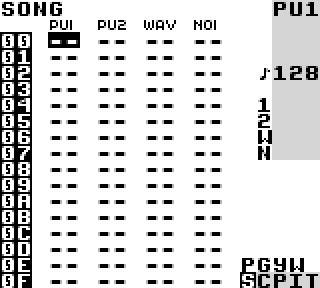
\includegraphics{song} }
\caption{Song Screen}
\label{fig:song}
\end{figure}

Little Sound Dj starts up in the song screen.
The four columns \textsc{PU1, PU2, WAV} and \textsc{NOI} represent the four Game Boy sound channels.
There are two pulse wave channels, one custom wave channel and one noise channel.
Use the D-pad to move the cursor from channel to channel.

\begin{figure}[hbtp]
\centering
\fbox{ 
\includegraphics[width=2.5cm]{map} }
\caption{Screen Map}
\label{fig:map}
\end{figure}

Little Sound Dj has nine screens, arranged in a map shown in the
bottom right of the screen (figure~\ref{fig:map}). 

The most useful screens are placed in the middle row, ordered by level of detail. 
The song, chain and phrase screens are used for sequencing, and work together in a tree-structure
fashion.  The song contains chains, each chain contains phrases, and each phrase contains notes.
They are followed by the instrument and table screens, which are used to create sounds.

To move between the screens, press \textsc{select+cursor}.

\section{Making Your First Sounds}
Navigate to the song screen, and move the cursor to the \textsc{pu1} column. Tap the \textsc{a} button,
and a new chain ``00'' will appear.
Edit the chain by pressing \textsc{select+right} to enter the chain screen.
There, tap \textsc{a} to insert a new phrase, then press \textsc{select+right} to go to the phrase screen.

\begin{figure}[hbtp]
\centering
\fbox{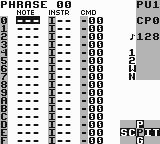
\includegraphics{phrase}}
\caption{Phrase Screen}
\label{fig:phrase1}
\end{figure}

In the phrase screen, you can enter notes to be played back. Move the cursor to the note
column and press \textsc{a} to enter a note. The text C-2 will appear: C being the note, and 2 the
octave. Press \textsc{start} to play the phrase. Notice how the phrase is played back from
top to bottom. You can change the note by holding \textsc{a} and pressing the
D-pad. \textsc{a+left/right} changes the note, and \textsc{a+up/down} changes octave.

Now, try to move the cursor and insert notes on other steps.
To delete a note, press \textsc{a} while holding \textsc{b}.
When you have finished listening, press \textsc{start} again to stop the phrase.

The clean pulse sound might get dull after while. Let's move on to the instrument
screen by pressing \textsc{select+right}.

\begin{figure}[hbtp]
\centering
\fbox{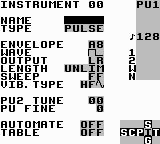
\includegraphics{instr-pulse}}
\caption{Instrument Screen}
\label{fig:instr}
\end{figure}

In the instrument screen, we can make the sound a little bit more interesting.
Try changing the \textsc{env.} and \textsc{wave} fields by moving the cursor there and pressing \textsc{a+left/right}.
As an example, changing the \textsc{env.} setting to \texttt{83} should make the sound shorter.
Press \textsc{start} again to hear the changes as you make them!

The \textsc{type} field sets the instrument type. Instrument types are specific for
channels -- \textsc{pulse} instruments should only be played back in the pulse channels, \textsc{wave} and \textsc{kit}
instruments in the wave channel, and \textsc{noise} instruments in the noise channel.

Let's try out the sampled drum kits. Now, we have to change channel to the wave channel.
Go back to the song screen, move the cursor over to the wave channel, and create a new
chain and a new phrase by tapping \textsc{a}.
Enter a note by tapping \textsc{a}, then \textsc{select+right} to edit the instrument.
Change the instrument type to \textsc{kit} by pressing \textsc{a+right} on the type field,
then go back to the phrase screen. Now, you should be able to enter drum sounds the same way
you entered notes before.

To create new chains and phrases, move the cursor to an empty step in song or chain screen and tap \textsc{a} twice.

\section{Hexadecimal Number System}

Little Sound Dj uses hexadecimal numbers. While the usual decimal number system uses ten digits, 0-9, hexadecimal has 16 unique symbols: the digits 0 to 9, followed by the letters A to F. For clarity, this manual will mark hexadecimal values with a \$ sign.
As an example, let's print a table of numbers -- first with decimal digits, then with
hexadecimal digits\ldots

\begin{figure}[hbtp]
\centering

\begin{tabular}{r|r|r|r|r|r|r|r|r|r|r}
 Decimal & 1 & 2 & 3 & 4 & 5 & 6 & 7 & 8 & 9 & 10 \\
\hline
 Hexadecimal & \$1 & \$2 & \$3 & \$4 & \$5 & \$6 & \$7 & \$8 & \$9 & \$A \\
\end{tabular}

\begin{tabular}{r|r|r|r|r|r|r|r|r|r|r}
 Decimal & 11 & 12 & 13 & 14 & 15 & 16 & 17 & 18 & 19 & 20 \\
\hline
 Hexadecimal & \$B & \$C & \$D & \$E & \$F & \$10 & \$11 & \$12 & \$13 & \$14  \\
\end{tabular}

\end{figure}

Note that the hexadecimal and decimal values are really equal; just the representations differ.
The reason to use the hexadecimal system here is to save screen space; with hexadecimal
numbers, it is possible to represent every byte value using no more than two digits. (The
value range is 0 to 255 -- that is, \$0 to \$FF.)

Representing negative numbers with two digits only can be a problem. In Little Sound Dj,
the numbers are wrapping. That means, when subtracting one from the smallest possible
number (\$0), it will jump to the highest possible value (\$FF). So \$FF can represent -1 as well as 255, depending on the situation.

If this does not make sense -- please don't worry too much -- it will become clear as you spend time with the program.

\section{Initial Troubleshooting}

Does your cartridge not start, crash, or act strange in other ways? Here are some things to try.

\begin{itemize}
	\item To avoid losing songs, always use fresh batteries. Replace as soon as the red light on your Game Boy gets faint, or the screen gets dim.
	\item Clean cartridge pins using a cotton swab and alcohol.
	\item Re-insert the cartridge a couple of times to remove oxide.
	\item Make sure that the cartridge is firmly plugged in. Sometimes it can help to put a piece of tape on the cartridge to give it a snug fit.
	\item Do a full reset of the cartridge memory. This is done by pressing \textsc{select+a+b} on the \textsc{load/save file} button in project screen.
	\item Certain Game Boy Advance/Nintendo DS cartridges do not work with Little Sound Dj. If you have problems with such a cartridge, try one of the Little Sound Dj builds named ``Goomba''.
	\item Search for help on the Little Sound Dj Wiki (\url{http://wiki.littlesounddj.com}) or ask in the Facebook group.
\end{itemize}

\chapter{The Screens}
Little Sound Dj has nine screens, laid out in a \begin{math} 5 \times 3 \end{math} screen map.

\section{Screen Map}

\begin{figure}[htbp]
\centering
\begin{tabular}{|c|c|c|c|c|}
	\cline{0-4}
	\multicolumn{2}{|c|}{} & \multicolumn{2}{|c|}{} & \\
	\multicolumn{2}{|c|}{Project} & \multicolumn{2}{|c|}{Synth} & Wave \\
	\multicolumn{2}{|c|}{} & \multicolumn{2}{|c|}{}  &\\
        \cline{0-4}
        & & & & \\
        Song & Chain & Phrase & Instr. & Table \\
        & & & & \\
        \cline{0-4}
        \multicolumn{5}{|c|}{} \\
        \multicolumn{5}{|c|}{Groove} \\
        \multicolumn{5}{|c|}{} \\
        \cline{0-4}
\end{tabular}
\end{figure}

The song, chain and phrase screens are used for composing music. The wave, synth,
instrument and table screens are used for making sounds.
Project screen contains project settings, and groove screen controls sequencer timing.
\footnote{There are also three hidden
screens, not shown on the map: The file, word and help screens. We will get back to these later.}

Most time is usually spent in the middle row, as that is where the composing is done.

Move between the screens using \textsc{select+cursor}. Synth and wave screens are overlaid; switch between them by pressing \textsc{select+right}.

\section{Starting and Stopping}

When pressing \textsc{start} in the song screen, Little Sound Dj plays all four
channels. When pressing \textsc{start} in other screens, Little Sound Dj plays the
channel that is being edited.
To start all four channels from some other screen than the song screen,
press \textsc{select+start}.

\section{Song Screen}

\begin{figure}[hbtp]
\centering
\fbox{ 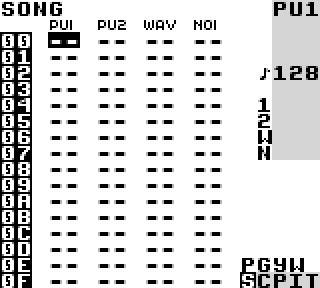
\includegraphics{song} }
\caption{Song Screen}
%\label{fig:song}
\end{figure}

The song screen is the highest level of the sequencer. This is where songs are arranged.
It has four columns, one for each channel. The columns contain lists of chains to be played top-down.

A list of key presses can be found in the help screen.


\includegraphics[width=0.8cm]{tip}TIP!
\begin{itemize}
	\item \textit{Press \textsc{b+a} on an empty step to pull up down-below chains.}
	\item \textit{To quickly jump between rows, mark them with \textsc{b,b,b} then jump with \textsc{b+up/down}.}
\end{itemize}

\section{Chain Screen}
A chain holds a list of phrases to be played back. It can represent for example a melody or a bass line. Each phrase has an optional transpose.

Chains can be reused freely between channels. It is particularly useful to play a chain in both pulse channels.

A list of key presses can be found in the help screen.

\begin{figure}[hbtp]
\centering
\fbox{ 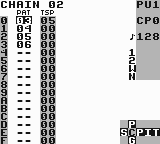
\includegraphics{chainexample} }
	\caption{This chain plays phrase 3 transposed by 5 semitones, followed by phrases 4-6 without transpose.}
\end{figure}

\section{Phrase Screen}

\begin{figure}[hbtp]
\centering
\fbox{ 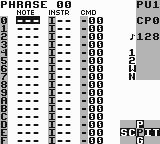
\includegraphics{phrase} }
\caption{Phrase Screen}
%\label{fig:phrase}
\end{figure}

The phrase screen is where you enter notes. It has four columns: note, instrument, command and command value.

Phrases are shared between channels; that is, any phrase may be played back on any channel. A phrase might however sound very different depending on which channel it is played back on. As an example, if a phrase plays a melody using a pulse instrument, it will probably sound good in the pulse channels but strange in the other channels.

The note column looks different depending on instrument. Usually it shows note and octave, but instruments that play back samples (\textsc{kit}, \textsc{speech}) show sample names instead. Noise instruments show either a byte value (for 15-bit noise) or note and octave (for 7-bit noise).

The instrument column selects instrument. Press \textsc{select+right} to edit an instrument in the instrument screen.

The command column is used to add commands. Each command has a special functionality. For example, the H command hops to next phrase. Tap \textsc{A,A} on any command for quick-help on what it does.


\includegraphics[width=0.8cm]{tip}TIP!
\begin{itemize}
    \item \textit{To change note without retrig, cut the instrument with \textsc{b+a}.}
    \item \textit{Mute kit note columns by pressing \textsc{a+right} until \textsc{off} appears. (Only works for kits with fewer than 15 samples.)}
\end{itemize}

\section{Instrument Screen}

\begin{figure}[hbtp]
\centering
\fbox{ 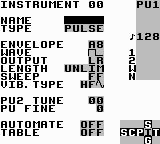
\includegraphics{instr-pulse} }
\caption{Instrument Screen}
\label{fig:instr2}
\end{figure}

There are five instrument types:

\begin{description}
\item[\textsc{pulse}] Makes pulse waves. Used in pulse channels 1 and 2.
\item[\textsc{wave}] Plays waves from the synth and wave screens. Used in the wave channel.
\item[\textsc{kit}] Plays samples from ROM. Used in the wave channel.
\item[\textsc{noise}] Makes pitched 7-bit or 15-bit noise. Used in the noise channel.
\item[\textsc{speech}] Instrument 40 is for speech and is used in the wave channel. Read more about speech in chapter \ref{speech-chapter}.
\end{description}

Change instrument type by pressing \textsc{a+cursor} on the \textsc{type} field.

Instruments don't automatically play in a matching channel. You have to make sure the instrument type matches the channel you are using. For example, to use the kit instrument, first make sure that you are in the wave channel.

\subsection{Instrument Parameters}
\label{general-instrument-parameters}

These parameters are used in most instrument types:

\begin{description}
	\item[\textsc{name}] Tap \textsc{a} to name the instrument. Useful for keeping instruments organized. When selecting instrument in phrase screen, this name is shown in the border.
	\item[\textsc{type}] Instrument type.
	\item[\textsc{length}] Sound length.
	\item[\textsc{output}] Send the sound to left/right/both/none speakers. (Use the headphone output to hear the difference!)
    \item[\textsc{pitch}] Controls the behavior of \textsc{p}, \textsc{l} and \textsc{v} commands. \textsc{A+u/d} switches pitch update speed: \textsc{fast} updates pitch at 360 Hz; \textsc{tick} updates pitch every tick; \textsc{step} is like \textsc{fast} except that \textsc{p} does pitch change instead of pitch bend; \textsc{drum} is like \textsc{fast} with logarithmic fall-off, useful for \textsc{p} kicks. \textsc{a+l/r} changes vibrato shape between downwards triangle, saw and square, and upwards triangle, saw and square.
    \item[\textsc{transp.}] When \textsc{on}, the pitch may be affected by project and table transposes.
    \item[\textsc{cmd/rate}] Slows down \textsc{c} and \textsc{r} commands.
        Also affects \textsc{p} and \textsc{v} commands when \textsc{pitch} is set to \textsc{tick}.
        0=fastest, F=slowest.
    \item[\textsc{table}] Selects a table to run when playing notes. To edit the table, press \textsc{select+right}. To create a new table, press \textsc{a,a}. To clone the table, press \textsc{select+(b,a)}.
        Changing \textsc{play} to \textsc{step} makes Little Sound Dj step through the table, advancing one step every time the instrument is triggered.
\end{description}


\includegraphics[width=0.8cm]{tip}TIP!
\begin{itemize}
	\item \textit{In the instrument screen, tap \textsc{A,A} on any parameter for quick-help on what it does.}
\end{itemize}

\subsection{Pulse Instrument Parameters}
\label{detune}

\begin{figure}[htpb]
	\begin{center}
\fbox{ 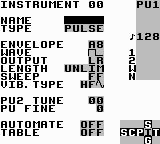
\includegraphics{instr-pulse} }
	\end{center}
	\caption{Pulse Instrument Screen}
	\label{fig:instr-pulse}
\end{figure}

\label{pulse-adsr}
\begin{description}
	\item[\textsc{env.}] Three amplitude envelope control values. For each value, first digit sets amplitude, and second digit sets the speed to rise or fall to the next amplitude. Speed 1 is fastest, F is slowest, 0 means hold. As an example, \textsc{env.} 32/AD/10 creates an envelope with fast attack from amplitude 3 to A, slow decay to amplitude 1, then infinite sustain, as shown in figure~\ref{fig:adsrexample}.
	\item[\textsc{wave}] Wave type.
	\item[\textsc{sweep}] Frequency sweep, useful for bass drum and percussion. The first digit sets time, the second sets pitch increase/decrease. Only works on the first pulse channel. 
\end{description}

\begin{figure}[hbtp]
\centering
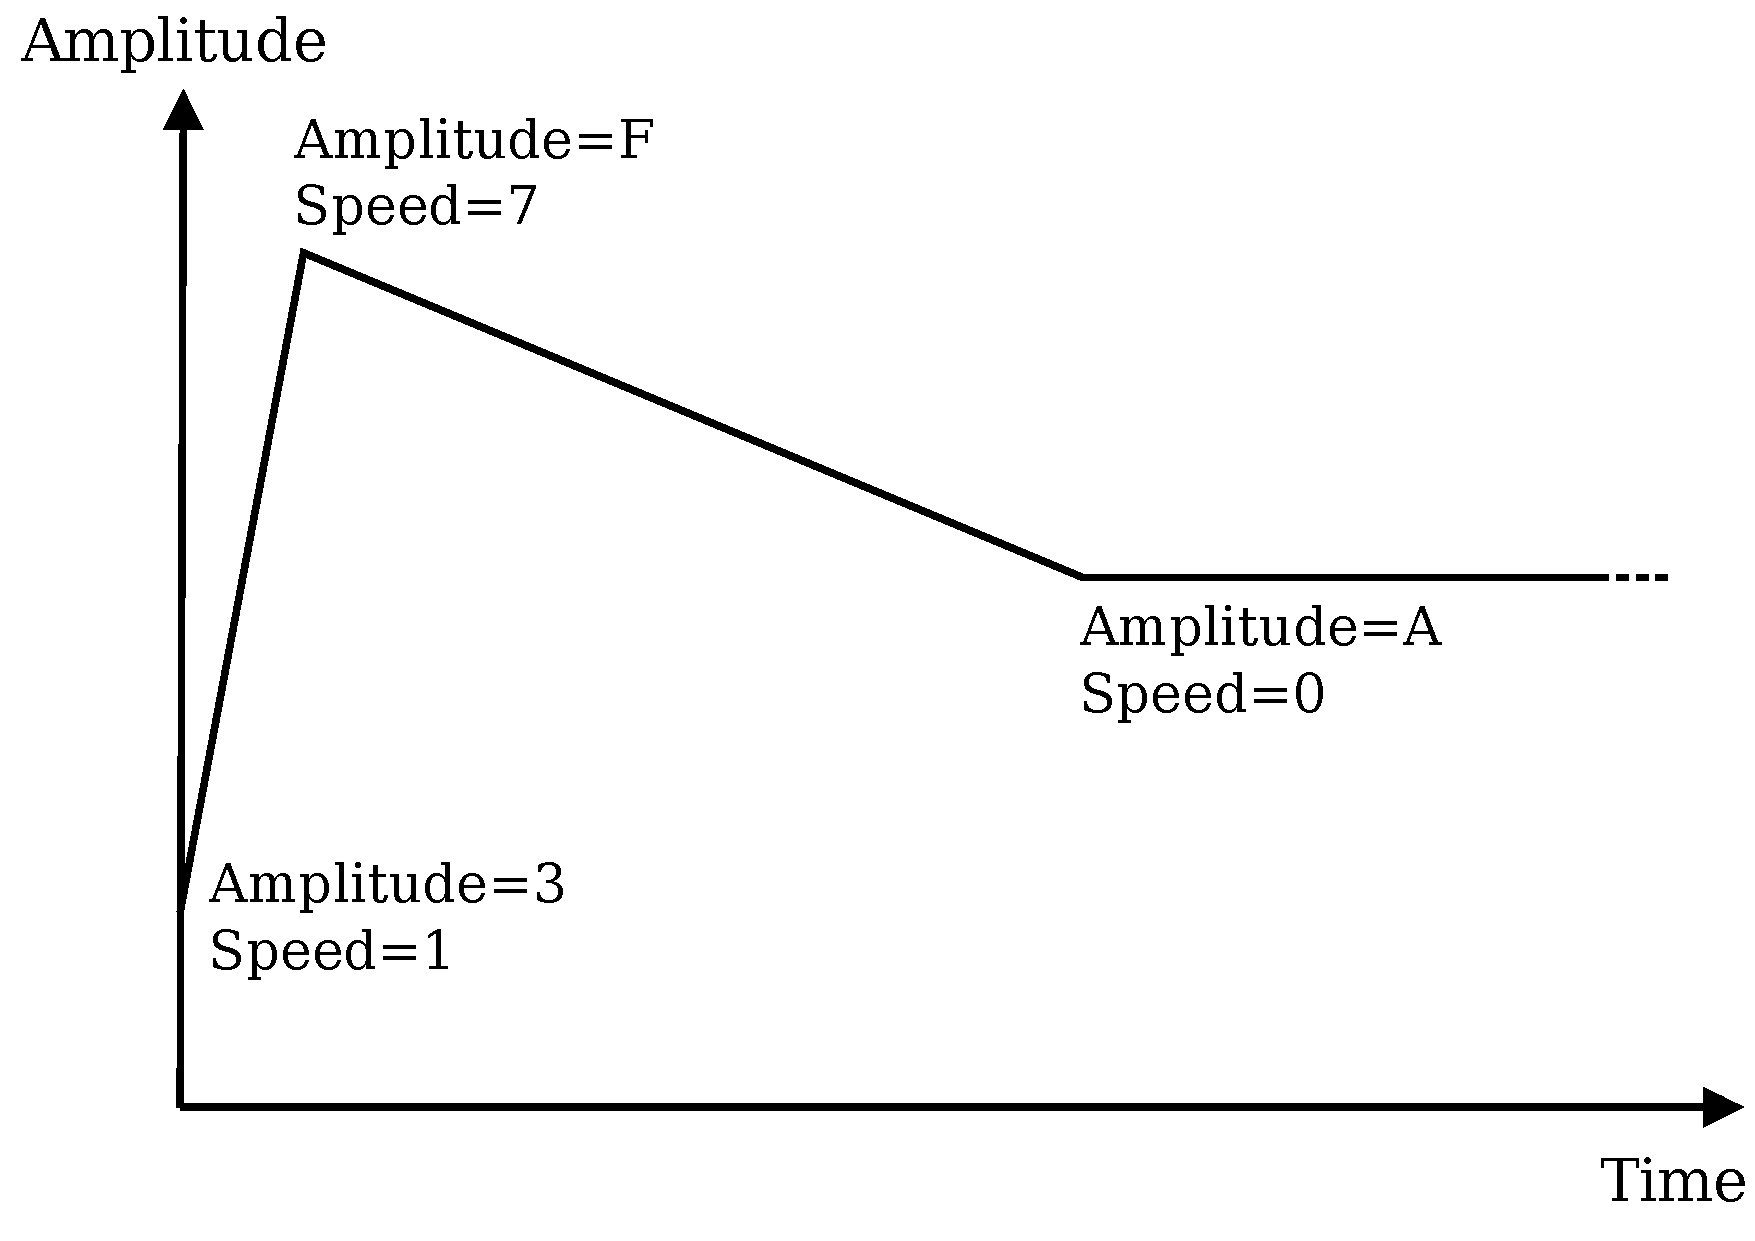
\includegraphics[width=7cm,angle=-90]{adsrexample} 
	\caption{Amplitude envelope example. \textsc{Env.}=32/AD/10.}
\label{fig:adsrexample}
\end{figure}

The detune settings create interesting phase effects when the same phrase is played on both pulse channels:

\begin{description}
	\item[\textsc{pu2 tsp.}] Transpose pulse channel 2.
	\item[\textsc{finetune}] Detune pulse channel 1 downwards, channel 2 upwards.
\end{description}

\subsection{Wave Instrument Parameters}

The wave instrument plays back synth sounds generated in the \textsc{synth} screen.

\begin{figure}[hbtp]
	\begin{center}
		\fbox { 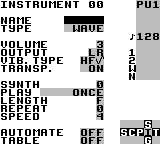
\includegraphics{instr-wave} }
	\end{center}
	\caption{Wave Instrument Screen}
	%\label{fig:instr-wave}
\end{figure}

\begin{description}
    \item[\textsc{volume}] Set amplitude (0=0\%, 1=25\%, 2=50\%, 3=100\%) and left/right output.
    \item[\textsc{finetune}] Detune the sound.
    \item[\textsc{wave}] Select the wave to play back. Waves are edited in the \textsc{wave} screen. When \textsc{play} is set to some other value than \textsc{manual}, this parameter is replaced by \textsc{synth}.
    \item[\textsc{synth}] Select the synth sound to play back. To edit the synth sound being used, press \textsc{select+up} to go to the \textsc{synth} screen. To use a new synth, tap \textsc{a} twice. To clone the synth, press \textsc{select+(b,a)}.
    \item[\textsc{play}] How to play back synth sounds: \textsc{manual}, \textsc{once}, \textsc{loop}, or \textsc{pingpong}. With \textsc{manual}, only a single wave is played. To play through a synth sound in \textsc{manual} mode, use the \textsc{f} command to step through its waves.
	\item[\textsc{speed}] How fast the synth sound should be played back.
	\item[\textsc{length}] Controls the length of the synth sound.
	\item[\textsc{loop pos}] Sets the loop point of the synth sound.
\end{description}

\subsection{Kit Instrument Parameters}

\begin{figure}[hbtp]
	\begin{center}
	\fbox {	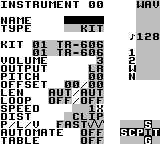
\includegraphics{instr-kit} }
	\end{center}
	\caption{Kit Instrument Screen}
	%\label{fig:instr-kit}
\end{figure}

\begin{description}
	\item[\textsc{kit}] Choose the sample kits to use. The first kit will be used in the left note column in the phrase screen; the second kit will be used in the right note column in the phrase screen.
    \item[\textsc{volume}] Set amplitude (0=0\%, 1=25\%, 2=50\%, 3=100\%) and output (left/right/both/off).
	\item[\textsc{finetune}] Pitch shift.
	\item[\textsc{offset}] Set the start loop point. If \textsc{loop} is \textsc{off}, this value can be used for skipping the initial part of a sound.
	\item[\textsc{len}] Sound length. \textsc{Aut} plays the sample to its end.
	\item[\textsc{loop}] Loop control. \textsc{Off}=don't loop, \textsc{on}=loop sound and start playing from \textsc{offset}, \textsc{atk}=loop sample and start playing from the beginning.
	\item[\textsc{speed}] Full speed or half speed.
	\item[\textsc{clip}] Selects what to do when the signal overshoots while mixing two kits. \textsc{Hard} is the default: Hard clamp the signal to the allowed 0-\$F range. \textsc{Soft} attenuates the signal to reduce distortion, giving a tape-like effect. \textsc{Fold} and \textsc{wrap} add digital distortion by folding or wrapping the signal around the 0 and \$F limits. Press \textsc{a+(left, left)} while \textsc{hard} is selected to mix the kits using raw memory contents.
\end{description}


\includegraphics[width=0.8cm]{tip}TIP!
\begin{itemize}
\item \textit{To replace the default sample kits, use the lsdpatcher program.} \url{https://littlesounddj.com/lsd/latest/lsd-patcher/}
\end{itemize}

\subsection{Noise Instrument Parameters}
\label{noise-instrument-parameters}

\begin{figure}[htpb]
	\begin{center}
		\fbox { 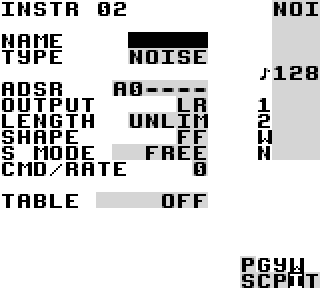
\includegraphics{instr-noise} }
	\end{center}
	\caption{Noise Instrument Screen}
	\label{fig:instr-noise}
\end{figure}

\begin{description}
	\item[\textsc{adsr}] See description of pulse ADSR (\ref{pulse-adsr}).
	\item[\textsc{pitch}] When set to \textsc{free}, pitch changes can randomly mute the sound. \textsc{Safe} avoids random mutes by restarting sound after any pitch change.
\end{description}

\subsection{Speech Instrument Parameters}

Read about the speech instrument in chapter \ref{speech-chapter}.

\section{Table Screen}

Tables are sequences of transposes, commands and amplitude changes which can be run at any speed and applied to any channel. By setting a table in the instrument screen, the table will start every time you play the instrument. This allows you to create more interesting sounds than would be possible using the instrument screen alone.

Tables contain six columns. The first column is the envelope column, used to create custom amplitude envelopes. Next is the transpose column, used to transpose the played note by a number of semitones. The other columns are command columns like the one in the phrase screen.

The default table speed of one tick per step can be changed using the G command. To view different tables, press \textsc{b+cursor}.


\includegraphics[width=0.8cm]{tip}TIP!
\begin{itemize}
	\item \textit{Press \textsc{select+right} on an A command in the phrase screen to edit that table. To jump back, press \textsc{select+left}.}
\end{itemize}

\subsection{Envelope Example}

The first digit in the envelope column sets the amplitude; the second digit sets for how many ticks the amplitude lasts.
To create an loop, set the first digit to the step you want to hop to, and the second digit to \textsc{H}.

\begin{figure}[htpb]
	\begin{center}
		\fbox{		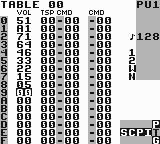
\includegraphics{table-amp} }
	\end{center}
	\caption{Table Envelope with Tremolo Effect}
	\label{fig:table-amp}
\end{figure}

The table in figure~\ref{fig:table-amp} creates a tremolo effect.

\subsection{Arpeggio Example}

\begin{figure}[htpb]
	\begin{center}
		\fbox{ 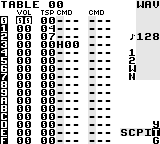
\includegraphics{table-arp}}
	\end{center}
	\caption{Table Transpose with Major Arpeggio}
	\label{fig:table-arp}
\end{figure}

A typical use for tables is to make arpeggios, which is a musical term for playing notes fast enough to sound like a chord. The table in figure~\ref{fig:table-arp} would form a major chord. Shorter arpeggios can also be made using the \textsc{c} command (see \ref{command-chord}).

\section{Groove Screen}

Grooves control by which speed your phrases and tables are played back. When used well, grooves will make your music sound more lively.

\begin{figure}[htbp]
	\begin{center}
		\fbox{ 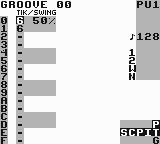
\includegraphics{groove} }
	\end{center}
	\caption{Groove Screen}
	\label{fig:groove}
\end{figure}

The sequencer is based on a time period called \emph{tick}, which is controlled by song tempo.
Ticks are very short: at 125 BPM, there are 50 ticks per second.
Higher tempo means faster ticks, and the other way around. 
In the groove screen, you can control for how many ticks phrase or table steps should last.
The groove in figure~\ref{fig:groove} would make the sequencer spend 6 ticks on every step.

\begin{figure}[htbp]
	\begin{center}
		\fbox{ 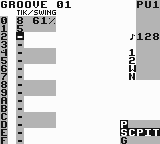
\includegraphics{groove-swing} }
	\end{center}
	\caption{Swing Example}
	\label{fig:groove-swing}
\end{figure}

You can also use grooves to create custom rhythms. The groove in figure~\ref{fig:groove-swing} would make even note steps last 8 ticks, and odd note steps last 5 ticks, creating a swing effect. Grooves can also be used to create triplets and other complex rhythms.

Groove 0 is the default groove for all phrases, but it is possible to switch to another groove using the G command.
This command also works in tables.

In the groove screen, select the groove you wish to edit by pressing \textsc{b+cursor}.


\includegraphics[width=0.8cm]{tip}TIP!
\begin{itemize}
	\item \textit{ \textsc{A+up/down} changes the swing percentage, while preserving the total number of ticks -- and thus, the resulting song speed -- constant. (Example: Original value is 6/6 = 50\%. Press \textsc{a+up}. Now the value changes to 7/5 = 58\%!) }
    \item \textit{ Press \textsc{select+up} on G commands to edit that groove. }
\end{itemize}

\section{Synth Screen}

The synth screen features a soft synthesizer that generates sounds to be played back by the wave instruments.
Each synth sound uses \$10 waves. Synth sound 0 uses waves \$00-\$0F, synth sound 1 uses waves \$10-\$1F, and so on. The generated synth sounds can be viewed in the wave screen (Section~\ref{wave-screen-section}).

In total, there are 16 synth sounds. Choose which one to edit by pressing \textsc{b+cursor}.

\begin{figure}[htbp]
	\begin{center}
		\fbox{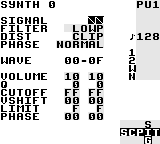
\includegraphics{synth}}
	\end{center}
	\caption{Synth Screen}
	\label{fig:synth}
\end{figure}

\subsection{Fixed Synth Settings}

\begin{description}
	\item[\textsc{signal}] Square, saw tooth, triangle or custom wave. \textsc{W.fx} uses a wave in range F0-FF as signal.
\item[\textsc{filter}] Low-pass, high-pass, band-pass or all-pass.
\item[\textsc{dist}] Distortion mode. \textsc{Clip} truncates the wave to \textsc{limit}, \textsc{fold} mirrors the wave around \textsc{limit}, \textsc{wrap} wraps around vertically.
\item[\textsc{phase}] \label{phase}
Compress the waveform horizontally. It is applied after filtering with \textsc{q} and \textsc{cutoff}. See figure \ref{fig:phasing} for examples.
\end{description}

\begin{figure}[hbtp]
	\centering
	\subfloat[Phase example. Original wave.]{
		\fbox{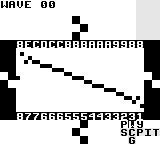
\includegraphics{wave}}
	}
	\qquad
	\subfloat[\textsc{normal} phasing. Compress horizontally, generate once.]{
	\fbox{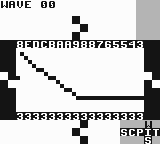
\includegraphics{phase-normal}}
	}

	\subfloat[\textsc{resync} phasing. Compress horizontally, loop.]{
		\fbox{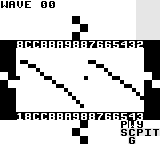
\includegraphics{phase-resync}}
	}
	\qquad
	\subfloat[\textsc{resyn2} phasing. Loop, but don't compress.]{
		\fbox{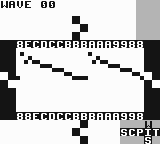
\includegraphics{phase-resyn2}}
	}
	\caption{Phase Examples}
	\label{fig:phasing}
\end{figure}

\subsection{Variable Synth Settings}

These settings control the first and last wave of the sound, with a smooth in-between fade.

\begin{description}
\item[\textsc{volume}] Signal volume.
\item[\textsc{q}] Resonance control. Boosts the signal around the cutoff frequency, to change how bright or dull the wave sounds.
\item[\textsc{cutoff}] Filter cutoff frequency.
\item[\textsc{vshift}] Shifts the signal vertically. See figure \ref{fig:vshift} for examples.
\item[\textsc{limit}] Limits the signal vertically using the \textsc{dist} mode.
\item[\textsc{phase}] 0 = no phase, \$1F = maximum phase. See figure \ref{fig:phasing} for examples.
\end{description}

\begin{figure}[htpb]
	\centering
	\subfloat[Vshift example. Original wave.]{
		\fbox{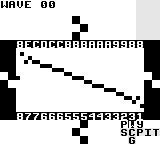
\includegraphics{wave}}
	}

	\subfloat[Vshifted signal. Vshift = 40, clip = wrap.]{
	\fbox{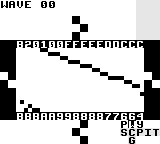
\includegraphics{vshift-40}}
	}

	\subfloat[Vshifted signal. Vshift = 80, clip = wrap.]{
		\fbox{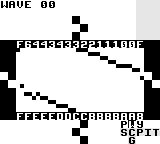
\includegraphics{vshift-80}}
	}
	\caption{Vshift Examples}
	\label{fig:vshift}
\end{figure}

\section{Wave Screen}
\label{wave-screen-section}

In the wave screen, you can view and edit the individual waveforms of the synth sounds. There are 16 synth sounds with 16 waves each. This means that synth sound 0 uses waves \$0-\$F, synth sound 1 uses waves \$10-\$1F, and so on.

To change selected values, press \textsc{up/down}. To flip selected values, press \textsc{a+cursor}. \textsc{B+cursor} navigates between different waves.

It is possible to modify multiple values at once, using the regular key presses:

\begin{description}
	\item[\textsc{select+b}] Start selection.
	\item[\textsc{select+b,b}] Select the entire wave.
	\item[\textsc{b}] Copy selection to clipboard.
	\item[\textsc{up/down}] Move selection up/down.
	\item[\textsc{a+left/right}] Flip selection horizontally. If no selection is made, draw a horizontal line.
	\item[\textsc{a+up/down}] Flip selection vertically.
	\item[\textsc{select+a}] Paste from clipboard.
\end{description}

\section{Project Screen}

\begin{figure}[htpb]
	\begin{center}
		\fbox{		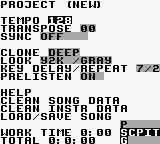
\includegraphics{project}}
	\end{center}
	\caption{Project Screen}
	\label{fig:project}
\end{figure}

The project screen (figure~\ref{fig:project}) contains settings that affect the entire program.

\begin{description}
	\item[\textsc{tempo}] Song tempo in BPM. It is possible to change the tempo either by pressing
\textsc{a+cursor}, or by tapping the \textsc{a} button in pace with the desired tempo. When being a
follower in sync mode, you can nudge the tempo by pressing \textsc{a+left/right}, something which
can be useful if devices have drifted out of sync.
	\item[\textsc{transpose}] Adjust the pitch of the pulse and wave instruments by the given number of semitones.
	\item[\textsc{sync}] Connects to other devices using the link port. Read all about sync settings in chapter \ref{sync-chapter}!

	\item[\textsc{clone}] Deep or slim chain cloning. Deep chain cloning will clone a chain's phrases, whereas slim cloning will re-use the old phrases. Read all about cloning in section \ref{cloning}!
	\item[\textsc{look}] Change the font and color set.
	\item[\textsc{key delay/repeat}] Set repeat delay and repeat rate of the Game Boy buttons.
	\item[\textsc{prelisten}] Play notes and instruments while entering them.

	\item[\textsc{help}] Enter help screen. The help screen contains a reference for button presses and a command list.
	\item[\textsc{clean song data}] Merge duplicate chains and phrases and clear unused ones. \label{clean-song-data}
	\item[\textsc{clean instr data}] Merge duplicate tables and clear unused instruments, tables, synths and waves.
	\item[\textsc{load/save song}] Enter file screen. \footnote{The file screen is only available for cartridges that have 1 Mbit SRAM or more. In case your cartridge doesn't have 1 Mbit SRAM, this button will be replaced with a \textsc{reset memory} button.}
\end{description}

The project screen also has two clocks.
The \textsc{worked} clock displays the time spent making the current song, in hours and minutes.
When playing, it is replaced by the \textsc{play} clock, which shows for how long the song has been playing.
The \textsc{total} clock shows how long the cartridge has been used in total, in days, hours and minutes.


\includegraphics[width=0.8cm]{tip}TIP!
\begin{itemize}
\item \textit{To replace the default fonts and palettes, use the lsdpatcher program.} \url{https://littlesounddj.com/lsd/latest/lsd-patcher/}
\end{itemize}

\subsection{Total Memory Reset}
\label{total-memory-reset}

Press \textsc{select+a+b} on \textsc{load/save file} to erase all songs and bring back the cartridge to its default state.
Generally, this is only useful if the cartridge got scrambled.

\section{File Screen}

\begin{figure}[htpb]
	\begin{center}
		\fbox{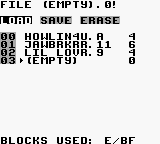
\includegraphics{file}}
	\end{center}
	\caption{File Screen}
	\label{fig:file}
\end{figure}

The file screen (figure~\ref{fig:file}) is entered by pressing the \textsc{load/save file} button in the project screen. It is used for saving the song you are working on to the storage memory. It can also be used to load songs from the storage memory to the work memory. The file screen allows you to keep up to 32 songs on one cartridge.

The file screen is only available for cartridges that have 64 kb SRAM or more.

\begin{description}
	\item[\textsc{file}] Shows the file name of the song you are working on. The exclamation mark (\textsc{!}) indicates when changes have been made to a song.
	\item[\textsc{load}] Load a song. Press \textsc{a}, select the file to load and press \textsc{a} again.
	\item[\textsc{save}] Save song. Press \textsc{a}, select the slot to save to and enter the file name.
	\item[\textsc{erase}] Erase a song. Press \textsc{a}, select the file to erase and press \textsc{a} again.
	\item[\textsc{blocks used}] Shows how much of the storage memory that is used. One block equals 512 bytes. The digits on the bottom are hexadecimal, meaning there is a total of \$BF * 512 = 97,792 available bytes.
\end{description}

Press \textsc{b} to return to the project screen.

\begin{figure}[hbtp]
	
\includegraphics[width=0.8cm]{tip}TIP!
	\begin{itemize}
		\item \textit{To manage songs, use the lsdpatcher program.} \url{https://littlesounddj.com/lsd/latest/lsd-patcher/}
	\end{itemize}
\end{figure}

\subsection{Song List}

The song list presents song name, version number and file size. When saving, the song is compressed, so the resulting file size will vary with different songs. To start working on a new song, load from the \textsc{(empty)} slot.


\includegraphics[width=0.84cm]{tip}TIP!
\begin{itemize}
    \item{While in the song list, press \textsc{select+a} to load a song without switching to the song screen, and \textsc{start} to start/stop songs. In this way, you can load and play songs without jumping back and forth between screens. This can be handy if you are playing a live show with prepared tracks and want fewer things to think about.}
\end{itemize}

\section{Border Information}

Various useful information is displayed in the screen border.

\begin{figure}[htpb]
	\begin{center}
	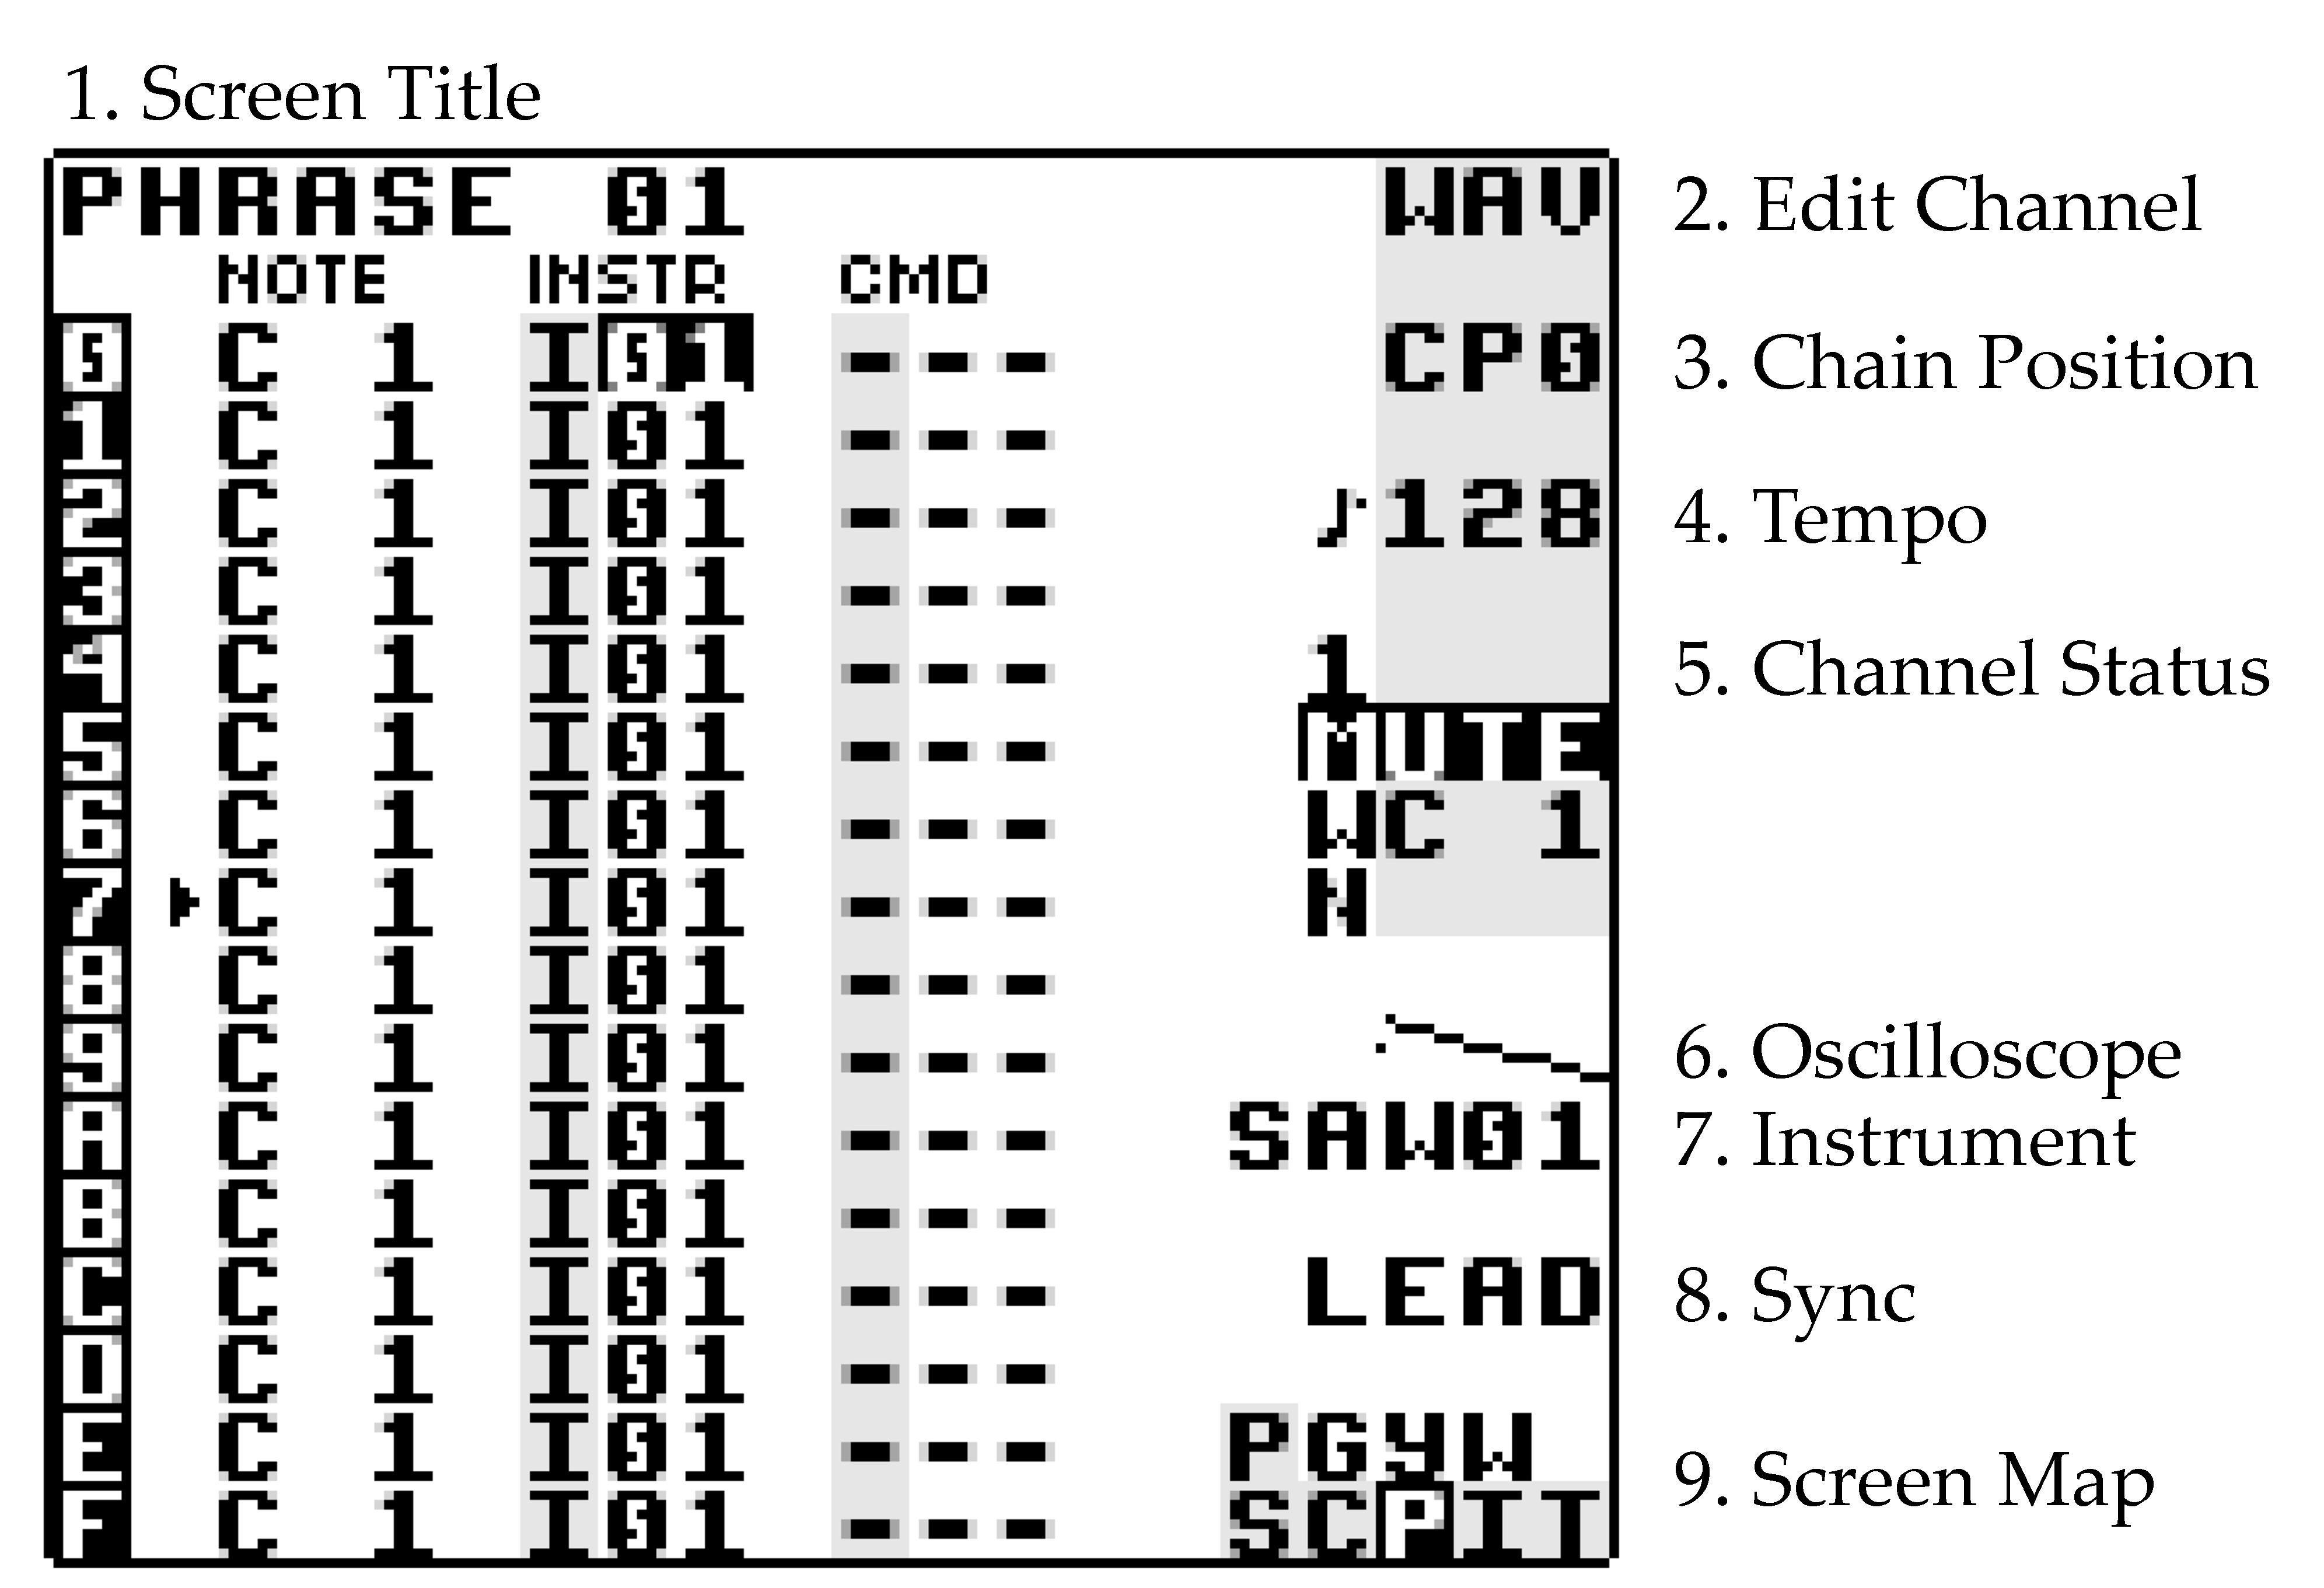
\includegraphics[width=11cm]{border}
	\end{center}
	\caption{Border Information}
	\label{fig:border}
\end{figure}

\begin{enumerate}
\item Screen title. Shows what is being edited.
\item The channel being edited, that is, the selected song screen column.
\item Chain position being edited.
\item Current tempo in beats per minute (BPM).
\item Shows what is being played on the channels. \textsc{Mute} appears when pressing \textsc{b+select} or \textsc{b+start}.
\item The waveform being played on the wave channel.
\item The name of the instrument being selected in the phrase screen.
\item Sync status.
\item Screen map.
\end{enumerate}



\chapter{Advanced Techniques}

\section{Copy and Paste} \label{copy-paste}

Little Sound Dj has a clipboard for temporary data storage. Pressing \textsc{b+a} will cut the value
under the cursor and store it on the clipboard. The value can then be pasted by pressing
\textsc{select+a}.

In most screens, it is possible to mark up blocks by pressing \textsc{select+b} and moving around
the cursor. When having marked up a block, it can be copied to the clipboard by pressing \textsc{b},
or cut to the clipboard by pressing \textsc{select+a}. The clipboard contents can then be pasted by
pressing \textsc{select+a}.

Some quick-mark button presses are implemented:
\begin{itemize}
\item \textsc{select+(b, b)} = quick-mark a column or row.
\item \textsc{select+(b, b, b)} = quick-mark an entire screen.
\end{itemize}

When having marked a block, you can change all data inside that block by pressing \textsc{a+cursor}. This can be used, for example, to transpose several notes quickly.

\section{Cloning}

Cloning is a shortcut that can save you much unnecessary copy and paste action. It allows you to create copies of chains, phrases, instruments and tables directly from the song, chain, phrase and instrument screens.

Let's say you have a melody in chain 00, and you want to continue the song with the same melody, but a little changed. Then you copy 00 \textsc{(select+b, b)} and paste one row down \textsc{(select+a)}, so you get:

\begin{verbatim}
 00 
 00 
\end{verbatim}

Now, place the cursor on the second 00, and press \textsc{select+(b, a)}.
You will now get a new chain (probably called 01) which is a copy of 00. Since it's a copy, you can play around with it as much as you want without touching 00.

\subsection{Deep vs. Slim-Cloning}

There are two different modes for cloning: slim-cloning and deep-cloning. You can select mode in the project screen.

If you slim-clone 00, Little Sound Dj makes a new chain 01 that
contains the same phrases as 00.

If you deep-clone 00, Little Sound Dj makes a new chain 00, and
also clones the phrases within 00 into 01. That way,
you can change 01's phrases without affecting 00.

The advantage of deep-cloning is that you have no risk of modifying old phrases by accident. The drawback is that it uses more phrases, so that you may run out of phrases faster. Also, your songs may take up more blocks when being saved using the file screen.

If you find yourself running out of phrases, try using \textsc{clean song data} in project screen. (Section \ref{clean-song-data}.)

\section{The Importance of Backups}

Some wise words from many peoples hard-earned experience: If you use Little Sound Dj on a Game Boy cartridge, it might be a good idea to examine backup options like the Transferer or the MegaMemory Card. Game Boy cartridges are often rather unstable, as they are depending on an internal battery that is likely to run out sooner or later. If you are serious about your music, you should do regular backups, or at least try to record your songs once in a while.

\section{Muting, Soloing and Panning on the Fly}

It is always possible to mute a channel temporarily by pressing \textsc{b+select}. If the \textsc{b} button is released before \textsc{select}, the channel will stay muted until \textsc{b} is pressed again. 

Correspondingly, a channel can be played solo by pressing \textsc{b+start}. If the \textsc{b} button is released before \textsc{start}, the other channels will stay muted. If the \textsc{start} button is released first, all channels will be turned on again.
 
It is also possible to pan channels left or right, by pressing \textsc{b+left/right} in the song screen.

\section{Live Mode}

 The live mode is a special flavor of the song screen. It can be reached by pressing \textsc{select+left} while in the song screen. In the live mode, it is possible to start and stop playing chains one by one. In contrast to the usual song screen, the different channels can be started and stopped independently. It is also possible to jump between different song positions while playing, without causing audio glitches or lost synchronization.

To play a chain, move the cursor to the chain and press \textsc{start}. To stop playing a chain, go to that channel and press \textsc{select+start}. If another chain is already playing, the starts and stops will be queued until that chain has been played through. If you want to queue until the next phrase end instead, tap \textsc{start} twice to speed up the switch.

To switch back to song mode from live mode, just press \textsc{select+left} while in the song screen.


\includegraphics[width=1cm]{tip}TIP!
\begin{itemize}
        \item \textit{To start or stop several chains at once, mark them before pressing \textsc{start} or \textsc{select+start}. (Marking is described in section \ref{copy-paste}.)}
	\end{itemize}

\subsection{Chain Loops}

 Using chain loops is a useful live mode technique. This technique is based on the fact that the song sequencer (when being in the live mode) won't rewind the song position all the way up to the first song sequencer step when encountering end of track; instead, it stops rewinding as soon as it encounters an empty step.

\begin{figure}[htpb]
	\begin{center}
	\fbox{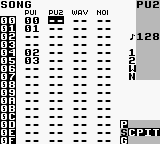
\includegraphics{chainloop}}
	\end{center}
	\caption{Chain Loop Example}
	\label{fig:chainloop}
\end{figure}

Example: We have a setup that looks like figure~\ref{fig:chainloop}.

Assume that we start playing pulse channel 1 at song position 4. The player will now loop chains 2 and 3. Defining a number of such chain loops to alternate between would provide a good starting point for a live performance.

\section{Creating Synthetic Drum Instruments}

Creating good-sounding drum instruments without using the sampled drum kits might be a bit tricky, if you've had no prior experience with drum synthesis. Nevertheless, it's a very useful technique once you know it. Here are some starting-out ideas.

\begin{figure}[hbtp]
	\centering
	\subfloat[Bass Drum]{
		\fbox{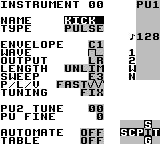
\includegraphics{instr-kick}}
	}
	\qquad
	\subfloat[Snare Drum]{
	\fbox{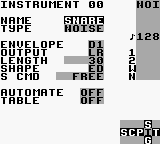
\includegraphics{instr-snare}}
	}

	\subfloat[Closed Hi-Hat]{
		\fbox{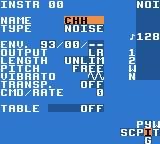
\includegraphics{instr-chh}}
	}
	\qquad
	\subfloat[Open Hi-Hat]{
	\fbox{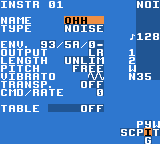
\includegraphics{instr-ohh}}
	}

	\subfloat[Cymbal]{
		\fbox{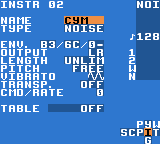
\includegraphics{instr-cym}}
	}
	\qquad
	\subfloat[Snare Drum Table]{
	\fbox{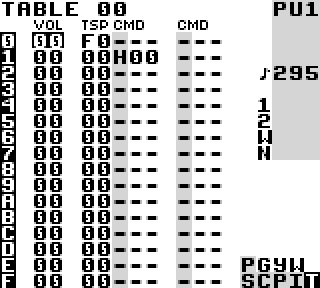
\includegraphics{table-snare}} \label{fig:table-snare}
	} 

	\caption{Synthetic Drum Instruments}
	\label{fig:instr-examples}
\end{figure} 

\subsection{Bass Drum}

Use pulse channel 1 for creating bass drum sounds. The amplitude envelope should have a strong attack and fast decay - try setting it to \$C1. Wave should be 50-50 high/low, even though other waves can be used for making the instrument sound more distorted. The sweep value is maybe the most important part in creating a successful kick instrument. It should have a high initial frequency and decay. Try setting it to a value of \$E3, and playing the instrument at note C-6. For a more snappy sounding kick, try experimenting with the envelope and length parameters.

It is also possible to use the noise channel for creating bass drums. Feel free to experiment around.

\subsection{Snare Drum}

Use the noise channel for creating snare drum sounds. The amplitude envelope should have a strong attack and fast decay - try setting it to \$C1. Use the length parameter to create more snappy sounding snares. The shape parameter can be used for adjusting the timbre - shape values close to \$EC might prove useful. 

\subsection{Hi-Hats and Cymbals}

Hi-hats are created using the noise channel. Use a shape value of \$FF for selecting a timbre with high frequency content. Change the envelope and length parameters for creating the desired amplitude envelope. For emulating cymbals, use a shape value near \$EE to create a somewhat rougher timbre.

\subsection{Taking Advantage of Tables}

For adding that extra punch to snares, you can use a table that uses the transpose column to change the noise shape rapidly. (See figure~\ref{fig:table-snare}.) 




\chapter{Overview of Key Presses}

This is an overview of key presses valid in the phrase screen. Most will work in other screens, too.

%\section{Key Presses}

\begin{description}

\subsubsection{Editing Notes}

\item[\textsc{a}] insert note on empty step

\item[\textsc{a+right}] note up
\item[\textsc{a+left}] note down
\item[\textsc{a+up}] octave/+10 up
\item[\textsc{a+down}] octave/-10 down

\item[\textsc{b+a}] cut note to clipboard

\subsubsection{Marking blocks}
\item[\textsc{select+b}] start marking
\item[\textsc{select+(b, b)}] mark row
\item[\textsc{select+(b, b, b)}] mark all

\subsubsection{When Having Marked a Block\dots}
\item[\textsc{a+left}] all marked down
\item[\textsc{a+right}] all marked up
\item[\textsc{a+up}] all marked octave/+10 up
\item[\textsc{a+down}] all marked octave/-10 down

\subsubsection{Copy/Paste Action}
\item[\textsc{b}] copy marked block to the clipboard
\item[\textsc{select+a}] cut the marked block to the clipboard

\item[\textsc{select+(b, b, b, b)}] copy the entire screen to the clipboard
\item[\textsc{select+a}] paste from the clipboard

\subsubsection{Switching Phrases}
\item[\textsc{b+left}] view the phrase in the leftmost channel
\item[\textsc{b+right}] view the phrase in the rightmost channel
\item[\textsc{b+up}] view previous phrase in chain
\item[\textsc{b+down}] view next phrase in chain

\subsubsection{Start/Stop in Song Mode}

\item[\textsc{start}] start/stop playing this phrase
\item[\textsc{select+start}] start/stop playing all channels

\subsubsection{Start/Stop in Live Mode}
\item[\textsc{start}] start playing selected chain after next chain end
\item[\textsc{start, start}] start playing selected chain after next phrase end
\item[\textsc{select+start}] stop playing current chain when it ends
\item[\textsc{select+(start, start)}] stop playing current chain after next phrase end

\subsubsection{Muting and Soloing}
\item[\textsc{b+select}] mute this channel
\item[\textsc{b+start}] solo this channel
\end{description}




\chapter{Commands}

Commands can be used in phrases and tables for altering the sound. There is a lot of power hidden in the commands, so it is suggested that you skim through this chapter at least once to get an idea of what they can do for you.


\includegraphics[width=1cm]{tip}TIP!
\begin{itemize}
        \item \textit{Tapping \textsc{a} on a command letter will display a scrolling help text in the top of the screen. \textsc{a+cursor} can then be used to browse through the existing commands. The text can be paused by holding \textsc{select}.}
	%\marginpar{
\includegraphics[width=1cm]{tip}TIP!}
	\end{itemize}

\section{A: Table Start/Stop}

Starts or stops tables in the current channel. Use the table number you want to start, or 20 for stopping.

\begin{description}
\item[A03] start table 3
\item[A20] stop table
\end{description}

\section{B: MayBe}

\subsection{In Phrases (MayBe Play Note)}

Controls how likely it is that the note
or sample(s) to the left will be played.
First digit sets probability for left kit,
second digit sets probability for notes
and right kit.

\begin{description}
    \item[B00] Never play note
    \item[B0F] Always play note/right kit sample
    \item[BF0] Always play note/left kit sample
    \item[B08] Play note/right kit sample about 50\% of the time
\end{description}

\subsection{In Tables (MayBe Hop)}

A hop that only happens sometimes.
First digit sets probability, second digit
sets destination row.

\begin{description}
    \item[BF5] Hop to row 5, 15 times out of 16
    \item[B84] Hop to row 4, about 50\% of the time
    \item[B03] Never hop to row 3
\end{description}

\section{C: Chord}

\subsection{For Pulse and Wave Instruments:}

\label{command-chord}
Produce chords by doing a simple arpeggio that extends the base note with the given semitones.

\begin{description}
\item[C37] plays a minor chord: 0, 3, 7, 0, 3, 7, 0, 3, 7, \ldots
\item[C47] plays a major chord: 0, 4, 7, 0, 4, 7, 0, 4, 7, \ldots
\item[C0C] plays 0, 0, C, 0, 0, C, 0, 0, C, \ldots
\item[CC0] plays 0, C, 0, C, 0, C, \ldots
\item[CCC] plays 0, C, C, 0, C, C, 0, C, C, \ldots
\item[C00] resets chord
\end{description}

\subsection{For Noise Instruments:}

Applies S command with the given value every second tick.

\section{D: Delay}

Delay the triggering of a note with the given number of ticks.

\section{E: Amplitude Envelope}

This command functions in two different ways, depending on which instrument type it is used on.

\subsection{For Pulse and Noise Instruments}
The first value digit sets the initial amplitude (0=min, \$F=max); the second digit sets the release (0,8: no change, 1-7: decrease, 9-\$F: increase).

\subsection{For Wave Instruments}
\begin{description}
\item[E00] volume 0\%
\item[E01] volume 25\%
\item[E02] volume 50\%
\item[E03] volume 100\%
\end{description}

\section{F: Wave Frame/Finetune}

\subsection{For Pulse Instruments:}
The first digit sets \textsc{pu2 tsp.}, the second \textsc{finetune}.
See section~\ref{detune}.

\subsection{For Kit Instruments:}
Modifies the sample position. \$00-\$7F steps forward, \$80-\$FF steps back.

\subsection{For Wave Instruments:}
Change the wave frame that's being played on the wave channel. This command is relative, meaning that the command value will be added to the current frame number. This can be used for playing through synth sounds manually.


\includegraphics[width=1cm]{tip}TIP!
\begin{itemize}
        \item \textit{Since a synth sound contains 16 (\$10) waves, issuing the command \textsc{F10} will in effect jump to the next synth sound.}
	%\marginpar{
\includegraphics[width=1cm]{tip}TIP!}
	\end{itemize}

\begin{description}
\item Example:
\item[F01] If wave frame 3 is being played, advance 1 frame and start playing frame number 4.
\end{description}

\section{G: Groove Select}

Select the groove to use when playing phrases or tables.

\begin{description}
\item Example:
\item[G04] select groove 4
\end{description}

\section{H: Hop}

H hops to a new play position. It can also be used to stop playing.

\subsection{H in Phrases}

\begin{description}
    \item[H00-H0F] Hop to next phrase. The digit sets destination phrase step.
    \item[H10-HFE] Hop back within the phrase. The first digit sets number of times to hop back, the second digit sets destination step.
    \item[HFF] Stop playing song (or channel, if in live mode).
\end{description}

\includegraphics[width=1cm]{tip}TIP!
\nolinebreak
\begin{itemize}
        \item \textit{If you want to compose in waltz time (3/4), put \textsc{H00} commands on step \textsc{C} in every phrase.}
\end{itemize}

\subsection{H in Tables}

In the table screen, H is used for creating table loops. The first digit sets how many times the hop should be done before moving on; 0 means ``forever.'' The second digit sets the table step to jump to. Loops can be nested; that is, you can have smaller loops inside bigger ones.

\begin{description}
\item Example:
\item[H21] hop twice to table position 1.
\item[H04] hop to table position 4 forever.
\end{description}

\section{K: Kill Note}

K instantly stops the sound, causing an audible click. If the click is not desired, better options might be E00 for wave channel and E11 for pulse and noise channels.

\begin{description}
\item Example:
\item[K00] kill note instantly
\item[K03] kill note after 3 ticks
\end{description}

\section{L: Slide}

Slides to the target note in the given duration. If the instrument's \textsc{pitch} setting is \textsc{tick}, the duration is given in ticks, otherwise in n/360 seconds.

Example:

\begin{verbatim}
  C-4 ---
  F-4 L40
  --- ---
  C-4 L10
\end{verbatim}

This will result in a slide that starts with C-4, bends to F-4, and then quickly bends back to C-4.

\subsection{L in Tables}

The L command also works in the left table command column, using the transpose column to set target note relative to the base note.

\begin{figure}[htbp]
	\begin{center}
		\fbox{\includegraphics{table-slide}}
	\end{center}
	% \caption{Synth Screen}
	% \label{fig:synth}
\end{figure}

Regular transposes and slides are added together independently. In the above example, step 0 transposes one octave up. In step 1, the L command starts sliding one octave down while keeping the transpose from step 0 unchanged. In step 2, the L command is allowed to play out while the transpose stays one octave up. After some time, L will stop one octave down, cancelling out the transpose and in practice returning to the base note.

\section{M: Master Volume}

This command changes the master output volume. The first digit modifies the left output, the second digit the right. The volume can either be set with an absolute value, or changed by a relative value.

Values 0-7 are used to specify absolute volumes. Values 8-\$F give the volume a relative change; 8 is no change, 9-\$B increase, \$D-\$F decrease.

\begin{description}
\item Examples:
\item[M77] maximize volume
\item[M08] minimize left volume, leave right volume unchanged
\item[M99] increase volume with 1 step
\item[MFE] decrease left volume with 1 step, right volume with 2 steps
\end{description}

\section{O: Set Output}

Pan channel to left, right, none or both outputs.

\section{P: Pitch Bend}

\subsection{For Pulse, Wave and Kit Instruments:}

Does a pitch change with the given speed. The behavior depends on the instrument's \textsc{pitch} setting:

\begin{description}
    \item[\textsc{drum}] Logarithmic pitch bend that updates at 360 Hz.
    \item[\textsc{fast}] Linear pitch bend that updates at 360 Hz.
    \item[\textsc{tick}] Pitch bend that updates every tick.
    \item[\textsc{step}] Immediate pitch change without bend.
\end{description}

Example:

\begin{description}
\item[P02] Pitch change up with speed 2.
\item[PFE] Pitch change down with speed 2. (\$FE=-2)
\end{description}

\subsection{For Noise Instruments:}

Applies S command with the given value every tick.

\section{R: Retrig the Latest Played Note}

Play the latest played note again. The first digit modulates the volume (0=no change, 1-7=increase, 8-\$F=decrease). The second digit sets a period for the retriggering, zero being the fastest and $E the slowest. Period $F means only retrig once.

\begin{description}
\item Example:
\item[R00] very fast retriggering
\item[R0F] retrigger once
\item[RF3] medium speed retriggering, decreasing amplitude (echo effect)
\end{description}

\section{S: Sweep/Shape}

This command has different effects for different instrument types.

\subsection{Pulse Instruments}

S modulates pitch, using the Game Boy hardware. It is useful for creating bass drums and percussion. The first digit affects pitch, the second changes pitch bend velocity.

Note: S has no effect when being used in pulse channel 2!

\subsection{Kit Instruments}

S changes the loop points. The first digit modulates the offset value; the second digit modulates the loop length. (1-7=increase, 9-\$F=decrease.) Used creatively, this command can be very useful for creating a wide range of percussive and timbral effects.

\subsection{Noise Instruments}

Alters noise shape (see section~\ref{noise-instrument-parameters}).
The command is relative, meaning that the digits are independently added to the active noise shape.

\section{T: Tempo}

Change the tick frequency so that the given \textsc{bpm} will be produced. The \textsc{bpm} setting will be accurate only if the active groove has 6 ticks per note step. If the groove has some other number of ticks per note step, the \textsc{bpm} value should be adjusted according to the formula
\begin{math}
lsdj\_bpm = (desired\_bpm \times ticks\_per\_step)/{6}
\end{math}.

\begin{description}
\item Example:
\item[T80] set tempo to 128 (\$80) \textsc{bpm}
\end{description}

\section{V: Vibrato}

Add vibrato. Not available for noise instruments. The vibrato speed and shape depends on the instrument's \textsc{pitch} setting.

\begin{description}
\item Example:
\item[V42] period=4, depth=2
\item[V00] reset vibrato
\end{description}

\section{W: Wave}

\subsection{For Pulse Instruments:}
Changes waveform.

\subsection{For Wave Instruments:}
The first digit sets synth sound speed, the second sets synth sound length. 0 = no change. The synth will be restarted if length is changed.

\section{Z: RandomiZe}

The Z command repeats the last non-Z command, adding a random number to the original command value. The Z value controls the maximum value of each digit to be added.

\begin{description}
\item Example:
\item[Z02] adds one of 0, 1, 2 to the original value.
\item[Z20] adds one of 0, 10, 20 to the original value.
\item[Z22] adds one of 0, 1, 2, 10, 11, 12, 20, 21, 22 to the original value.
\end{description}

Note: Randomize does not work with Hop, Groove and Delay commands at the moment.

\chapter{Synchronization}
\label{sync-chapter}

LSDj can synchronize with other devices through the link port, so that it is possible to run both in exactly the same tempo. Enable synchronization by changing the \textsc{sync} mode in the project screen.

\textsc{Important}: When running synchronized, use a groove based on 6 ticks/step. Otherwise, the resulting speed might be wrong.

\section{Game Boy to Game Boy Sync}

It is possible to sync two Game Boys running LSDj using a Nintendo Game Link cable.

\subsection{Activating LSDj Sync}

Make sure that both Game Boys are turned off. Connect the Game Boys using the link cable. Now, turn on the Game Boys, and go to the project screens. Set the \textsc{sync} mode to \textsc{lsdj} on both Game Boys.

\subsection{Song Play}

When in song mode, pressing \textsc{start} starts both Game Boys from the same song position. The Game Boy on which you pressed \textsc{start} is the one that sends sync signals; this is indicated by the text \textsc{lead} appearing in the right margin. The other Game Boy shows the text \textsc{sync}, indicating that it is receiving sync signals.

\subsection{Live Play}

Pressing \textsc{start} in live mode makes the Game Boy start like usual; also \textsc{lead}/\textsc{sync} texts indicate that sync signals are sent between the Game Boys. When pressing \textsc{start} on the following Game Boy, the text \textsc{wait} appears while it is waiting for a phrase start.

\subsection{Clipboard Transfer}

When two Game Boys are linked and not playing, copying groove, chain, phrase, instr, table, wave or synth data on one Game Boy will transfer the copied data so it can be pasted on the other Game Boy.

\subsection{Switching Lead while Playing}

In some cases, it can be useful to switch which Game Boy is the lead while playing. Do this by following steps:

\begin{enumerate}
    \item Set Game Boys to \textsc{lsdj} sync.
    \item Start playing.
    \item Set the following Game Boy to sync \textsc{off}.
    \item Stop lead Game Boy.
    \item Set the following Game Boy to sync \textsc{lsdj}. It now becomes the lead.
\end{enumerate}

\section{\textsc{Midi} Sync}

\textsc{Midi} sync requires a special \textsc{Midi} sync cable for Game Boy. For information on how to build a \textsc{Midi} to Game Boy adapter, please refer to the website at \url{https://www.littlesounddj.com}.

Usage: Plug in the sync device before turning on your Game Boy. Then, set LSDj to \textsc{Midi} sync mode. Pressing \textsc{start} will now make LSDj wait for and sync with any incoming \textsc{Midi} clock signals. LSDj should use grooves based on 6 ticks.

\begin{figure}[hbtp]
\includegraphics[width=0.84cm]{tip}TIP!
\begin{itemize}
        \item \textit{When LSDj is following, it is possible to temporarily play
slower or faster by pressing \textsc{a+left/right} on tempo in project screen. This can
be very useful when being hooked up to some external hardware that has drifted slightly out
of sync.}
	\end{itemize}
\end{figure}

\section{Analog In}

LSDj can sync to music equipment that sends analog sync signals. This sync mode has been tested with the Korg Volca series, but works with other gear too; you can find a list at \url{https://littlesounddj.wikia.com/wiki/Analog_Sync_Compatibility}.

A cable should be easy to make, since no particular electronics are needed: all it takes is to splice a Nintendo Game Link Cable and a 3.5 mm mini plug cable together. The wires should be connected as shown in the below diagram: GND goes to GND, CLK goes to CLK.

\includegraphics[clip=true,trim=0 0 460 250,angle=270,width=10cm]{analog-in}\\

As a clarification, the above diagram is looking at the cable, and the wires are probably not red and blue in reality.

Once the cable is built, connect it to the Game Boy serial port and the \textsc{sync out} of your synthesizer. In project screen, set LSDj to \textsc{analog} sync mode. The \textsc{ticks/step} setting controls how many LSDj ticks should be generated for each incoming sync signal. Depending on the synthesizer, it may be necessary to change this setting to make LSDj run at the right speed. For Korg Monotribe, it should typically be set to 6, whereas for Korg Volca, it should be C.

\section{Analog Out}

Analog Out works similar to Analog In, except that in this mode, LSDj is responsible for sending the sync signal. The cable is different from the one used for Analog In. Build it by connecting the wires as follows:

\includegraphics[clip=true,trim=0 0 460 250,angle=270,width=10cm]{analog-out}\\

As a clarification, the above diagram is looking at the cable, and the wires are probably not red and blue in reality. This cable should be connected to \textsc{sync in} of your synthesizer.

\section{Troubleshooting Cables}

When making cables, double and triple check that the wires are connected to the right pins. You will need a multimeter for probing the pins. If they are not connected exactly like they should, you can get cables that nearly work, but the sync is a little off. The most common problem is flipped pins; remember that the diagrams are looking at the cable, not from it!

\section{Keyboard Control}

The \textsc{keybd} sync mode allows connecting a PS/2 keyboard to the Game Boy and playing it like a piano. This can be fun for live shows and improvisation. For information on how to build a PS/2 keyboard to Game Boy adapter, please refer to the Wiki site: \url{https://wiki.littlesounddj.com}

The keyboard must be calibrated once is plugged in. To do this, go to the project screen, set sync mode to \textsc{keybd}, and press \textsc{A} on the \textsc{ps/2 delay} setting. Then, press the down arrow key on your PS/2 keyboard repeatedly until LSDj says \textsc{ok!}

To get sound when playing the keyboard, first go to phrase screen and move cursor to note column, or press \textsc{start} to play the keyboard while the song is running.

\subsection{Keyboard Note Layout}

\begin{figure}[htpb]
	\begin{center}
	\fbox{\includegraphics[width=10cm]{keybd-map}}
	\end{center}
	\caption{PC Keyboard Map}
	\label{fig:keybd-map}
\end{figure}

\begin{description}
\item[\textsc{space}] play using custom table
\item[\textsc{f1/f2}] octave down/up
\item[\textsc{f3/f4}] instrument down/up
\item[\textsc{f5/f6}] select custom table to assign to \textsc{space}
\item[\textsc{f8}] change pulse instrument playback channels (\textsc{PU1, PU2, PU1+2})
\item[\textsc{f9-f12}] toggle channel mute (switches on key press)
\item[\textsc{ctrl+(f9-f12)}] tap channel mute (switches on key press and release)
\item[\textsc{cursor movement keys}] move around cursor
\item[\textsc{enter}] play chain
\item[\textsc{ctrl+enter}] stop chain
\item[\textsc{page up/down}] \textsc{b+up/down}
\end{description}


\chapter{Speech Programming}
\label{speech-chapter}

\section{Introduction}

Little Sound Dj has 59 speech sounds, called allophones. By combining these sounds, it is possible to create any English word or phrase.

The speech instrument is locked to instrument number \$40 and can only be used in the wave channel. It contains 14 word slots, by default named W-0 to W-D.

\begin{figure}[htpb]
	\begin{center}
	\fbox{\includegraphics{speech}}
	\end{center}
	\caption{Speech Instrument Screen}
	\label{fig:speech}
\end{figure}
\begin{figure}[htpb]
	\begin{center}
	\fbox{\includegraphics{word}}
	\end{center}
	\caption{Example Word}
	\label{fig:word}
\end{figure}

To edit a word, press \textsc{select+right} to get to the word screen. The left column contains the allophones to be played, the right column sets their duration. The word in figure~\ref{fig:word} is supposed to say ``Little Sound Dj.''

To make the words easy to remember, rename them by tapping A in the speech instrument screen.

\section{Allophones}

\begin{itemize}
\item When selecting allophones, care about how they sound, not how they are spelled.
\item A sound may be different depending on its position within a word. For example, the K in ``coop'' will sound different from the K's in ``keep'' and ``speak''.
\end{itemize}

Allophones marked with * loop indefinitely.

\subsection{Short vowels}

\begin{description}
\item[*IH] sitting, stranded
\item[*EH] extent, gentlemen
\item[*AE] extract, acting
\item[*UH] cookie, full
\item[*AD] talking, song
\item[*AX] lapel, instruct
\end{description}

\subsection{Long vowels}

\begin{description}
\item[IY] treat, people, penny
\item[EY] great, statement, tray
\item[AY] kite, sky, mighty
\item[OI] noise, toy, voice
\item[UW1] after clusters with YY: computer
\item[UW2] in monosyllabic words: two, food
\item[OW] zone, close, snow
\item[AW] sound, mouse, down
\item[EL] little, angle, gentlemen
\end{description}

\subsection{R-colored vowels}

\begin{description}
\item[ER1] letter, furniture, interrupt
\item[ER2] monosyllables: bird, fern, burn
\item[OR] fortune, adorn, store
\item[AR] farm, alarm, garment
\item[YR] hear, earring, irresponsible
\item[XR] hair, declare, stare
\end{description}

\subsection{Resonants}
\begin{description}
\item[WW] we, warrant, linguist
\item[RR1] initial position: read, write, x-ray
\item[RR2] initial clusters: brown, crane, grease
\item[LL] like, hello, steel
\item[YY1] clusters: cute, beauty, computer
\item[YY2] initial position: yes, yarn, yo-yo
\end{description}

\subsection{Voiced fricatives}
\begin{description}
\item[VV] vest, prove, even
\item[DH1] word-initial position: this, then, they
\item[DH2] word-final and between vowels: bathe, bathing
\item[ZZ] zoo, phase
\item[ZH] beige, pleasure
\end{description}

\subsection{Voiceless fricatives}
\begin{description}
\item[*FF] fire, fox
\item[*TH] this, they
\item[*SS] sit, smile
\item[SH] shirt, leash, nation
\item[HH1] before front vowels: YR, IY, IH, EY, EH, XR, AE
\item[HH2] before back vowels: UW, UH, OW, OY, AO, OR, AR
\item[WH] white, whim, twenty
\end{description}

\subsection{Voiced stops}
\begin{description}
\item[BB1] final position: rib; between vowels: fibber, in clusters: bleed, brown
\item[BB2] initial position before a vowel: beast
\item[DD1] final position: played, end
\item[DD2] initial position: down; clusters: drain
\item[GG1] before high front vowels: YR, IY, IH, EY, EH, XR
\item[GG2] before high back vowels: UW, UH, OW, OY, AX; and clusters: green, glue
\item[GG3] before low vowels: AE, AW, AY, AR, AA, AO, OR, ER; and medial clusters: anger; and final position: peg
\end{description}


\subsection{Voiceless stops}
\begin{description}
\item[PP] pleasure, ample, trip
\item[TT1] final clusters before SS: tests, its
\item[TT2] all other positions: test, street
\item[KK1] before front vowels: YR, IY, IH, EY, EH, XR, AY, AE, ER, AX; initial clusters: cute, clown, scream
\item[KK2] final position: speak; final clusters: task
\item[KK3] before back vowels: UW, UH, OW, OY, OR, AR, AO; initial clusters: crane, quick, clown, scream
\end{description}

\subsection{Affricates}
\begin{description}
\item[CH] church, feature
\item[JH] judge, injure
\end{description}

\subsection{Nasal}
\begin{description}
\item[MM] milk, alarm, example
\item[NN1] before front and central vowels: YR, IY, IH, EY, EH, XR, AE, ER, AX, AW, AY, UW; final clusters: earn
\item[NN2] before back vowels: UH, OW, OY, OR, AR, AA
\end{description}




\chapter{The Sample Kits}


\xentrystretch{-0.05}
\tablehead{%
%\hline
\multicolumn{1}{l}{\bf{Machine}} &
\multicolumn{1}{l}{\bf{Year}} &
\multicolumn{1}{l}{\bf{Info}}
\\
}
%\tabletail{ \hline }
\tablelasttail{ \hline }
%\tablelasttail{ \multicolumn{3}{l}{} \\ \hline }
\begin{xtabular}{p{2.02cm}|l|p{7.8cm}}

\hline
SP0256-AL2 \linebreak
General Instruments 
& 1981 & 
\includegraphics[width=4.7cm]{sp0256al2}

The SP0256-AL2 Speech Processor IC contains a programmable digital filter that can be made to model a vocal tract. The 16k ROM stores both data and instructions. The pulse width modulated output can produce speech with a frequency range of 5kHz and a dynamic range of 42 dB. \\
\hline
TR-606 \linebreak Roland & 1981 & 
\includegraphics[width=5.8cm]{tr606}

The Roland TR-606 Drumatix is a programmable analogue drum machine. It was designed to couple with the TB-303 Bassline. The TR-606 has a very original sound and remains popular today. \\
\hline
TR-707 \linebreak Roland & 1984 & 
\includegraphics[width=5.8cm]{tr707}

The Roland TR-707 has the same functions as the TR-909 with all PCM sounds. Starting with this model, Roland began using an LCD display to show the rhythm matrix and tempo. \\
\hline
TR-727 \linebreak Roland & 1985 & 
\includegraphics[width=5.8cm]{tr727}

The Roland TR-727 is identical to the TR-707, with the exception that its sounds are Ethnic/Latin percussion. It is meant to complement a rhythm section, rather than be a main unit. \\
\hline
TR-808 \linebreak Roland & 1980 & 
\includegraphics[width=6.0cm]{tr808}

The Roland TR-808 has played a defining role for the 80's Hip Hop and Electro movement. It is still highly popular, thanks to its unmistakably original sounds. \\
\hline
TR-909 \linebreak Roland & 1983 & 
\includegraphics[width=5cm]{tr909}

The Roland TR-909 is one of the most popular drum machines ever. It has PCM sounds for cymbal and hi-hat, but all other instruments still come from analogue circuitry. The sounds are very useful for House and Techno music. \\
\hline
CR-78 \linebreak Roland & 1978 & 
\includegraphics[width=5cm]{cr78}

The Roland CR-78 is perhaps the most luxurious rhythm machine ever made. The guiro and tambourine are still unique as of today, and bass, snare and bongos sound very soft and rich. \\
\hline
CR-8000 \linebreak Roland & 1981 & 
\includegraphics[width=5cm]{cr8000}

The Roland CR-8000 was introduced after the TR-808 -- it has the same analog engine. The hi-hat sounds more realistic than older rhythm machines, but the hand clap sounds like an electric snare. \\
\hline
DR-55 \linebreak Boss & 1979 & 
\includegraphics[width=5.4cm]{dr55}

The Boss Dr. Rhythm range of drum machines is especially designed for guitar players who need a mobile drummer. The DR-55 is a simple analogue drum machine with a very rough and direct sound. \\
\hline
DR-110 \linebreak Boss & 1983 & 
\includegraphics[width=5.4cm]{dr110}

The DR-110, the successor of the DR-55, has analogue sound but is programmed digitally using a LCD rhythm matrix. It quite possibly has the best analogue handclap ever. \\
\hline
LinnDrum & 1982 & 
\includegraphics[width=6.1cm]{linndrum}

The LinnDrum originally sold for \$3,000 and about 5.000 units were produced. It provided the rhythm tracks of many 1980's hit records. \\
\hline
Rhythm Ace & 1967 & 
\includegraphics[width=5.2cm]{rhyace}

Ace Tone was the first company to produce electric rhythm boxes in Japan. In the UK, Bentley Pianos (who put stickers on all their products) distributed Ace Tone, and thus the machine is also known as the Bentley Rhythm Ace. \\
\hline
Tom \linebreak
Sequential \linebreak
Circuits & 1984 & 
\includegraphics[width=6.7cm]{tom}

The sounds are a bit dirty and harsh sounding, especially next to its older brother Drumtraks, but that also gives Tom its character. The snare sounds like nothing else on this planet - it's electric! \\
\hline
Acieed House & 1990's & 
\includegraphics[width=3.5cm]{smiley_gray}

This set of vocal samples was derived from a bunch of popular Acid House tracks. Can you dig it? \\

\hline
Animals \linebreak Bud Melvin & 2004 & 
\includegraphics[width=6.7cm]{kit-farm} 

The winner of the 2004 Animal Sample Compo. A great selection of domestic animals. \\
\end{xtabular}



\end{document}

